\documentclass{article}
\usepackage{amsmath,amssymb,amsthm,enumitem} % Some standard math packages.
\usepackage{titling} % Enables \setlength{\droptitle}
\usepackage{parskip} % Cleaner paragraph display
\usepackage[margin=1in]{geometry} % Adjusts margins.
\usepackage[utf8]{inputenc} % USe UTF-8 input encoding instead of default ASCII.
\usepackage[]{forest} % Draws trees.
\usepackage{fancyvrb} % Allows Verbatim sections with line numbers and such. Note the capital V.
\usepackage{pgfplots} % For drawing graphs
\usepackage{hyperref} % For hyperlinks
\pgfplotsset{compat=1.6}
\newcommand {\todo}[1] {{\textbf{\color{red}#1}}}

\title{CS 584 Research Project}
\author{ Dylan Laufenberg }
\date{June 5, 2018}

\begin{document}
\maketitle

\paragraph{Project topic} I will implement a variety of data structures that maintain total orders on their data, e.g. 2-3 trees, treaps, and skip lists; I will choose at least one deterministic structure as a reference and at least one randomized data structure for comparison. I will experimentally evaluate the rates of growth of their run times for insertions, searches, and deletions. Based on these data, I will discuss how the performance I observe compares to the predicted asymptotic performance.

\section{Introduction}
This paper aims to illuminate various facets of the relationship between asymptotic complexity and empirical performance of a range of related data structures. The vehicle for this exploration is a series of benchmarks of data structures that perform similar jobs in very different ways. These include binary search trees, treaps, and skip lists \todo{FINALIZE LIST OF DATA STRUCTURES}. For many tasks, they have the same asymptotic complexity, e.g. average complexity of $O(\log n)$ for search, insert, and delete operations, with worst-case complexity of $O(n)$ for each. This paper examines the performance characteristics of each and investigates how comparable the performance characteristics of these asymptotically equivalent data structures really are.

\section{Testing Methodology}
Gathering reliable data is, of course, of paramount importance to any data-based analysis. Since the analysis in this paper is based on benchmark data, the accuracy of the analysis hinges on the accuracy of the benchmarks themselves. The benchmarks included in this paper utilize the following measures to help ensure their accuracy:

\begin{itemize}
    \item To minimize the impact of timer error, CPU load spikes, and so on, each data point is the average running time of a large number of operations $k$, where $k \geq 100$.
    \item To minimize the impact of such large values of $k$, the overall sample sizes are suitably large, such that $n \geq 100 \cdot k$, where $n$ is the size of a data structure when the $k$ timed operations begin. In other words, the number of operations being timed is no larger than 1\% of the overall data structure at any point.
    \item When necessary for accuracy, multiple passes may be combined by taking the median or mean time of the running times for each value of $n$ being plotted.
    \item To prevent human error in transcribing graphs or plot data, all graphs are generated programmatically using the same function and included without modification.
\end{itemize}

\emph{Note that some of the graphs under \todo{TESTING DATA STRUCTURES SECTION NAME} necessarily disobey the above guidelines.}

\section{Project Files}
The Python 3 implementations included with this report are structured as follows:
\begin{itemize}
    \item datastructures/ --- contains the implementations of data structures benchmarked below, one per file.
    \item plots/ --- contains the output \LaTeX \ figures that the benchmark system produces, ready to \\include.
    \item pgfplot.py --- contains the PgfPlot class, which represents one \LaTeX \ figure to be produced. This class receives and stores all parameters that affect the figure, including plots to be produced.
    \item plot.py --- contains the Plot and BenchmarkPlot classes, which represent plots in a PGFPLOT graph. The Plot class may be used to produce arbitrary plots, whereas the BenchmarkPlot class receives benchmark parameters for one function and produces the corresponding plot.
    \item benchmark.py --- sets up and runs the benchmarks used in this document by creating PgfPlot objects and running them.
\end{itemize}

To run custom benchmarks, simply follow the examples in benchmark.py. All classes are thoroughly documented and commented.

\section{Data Structure Selection}
Many implementations exist for each of these data structures, since they are well-known. 

\section{Data Structure Implementations}
All credit for implementations go to the authors of the respective data structure implementations. All data structures used are cited here.

\begin{itemize}
    \item binarysearchtree.py --- Dylan Laufenberg (written as a naive reference for these benchmarks)
    \item pyskip.py --- taken from \url{https://github.com/toastdriven/pyskip}. Credit: Daniel Lindsley.
\end{itemize}

\todo{Charts here comparing different implementations of various data structures}

\newpage
\section{Testing TikZ Pictures}

\begin{figure}[h]
    \centering
    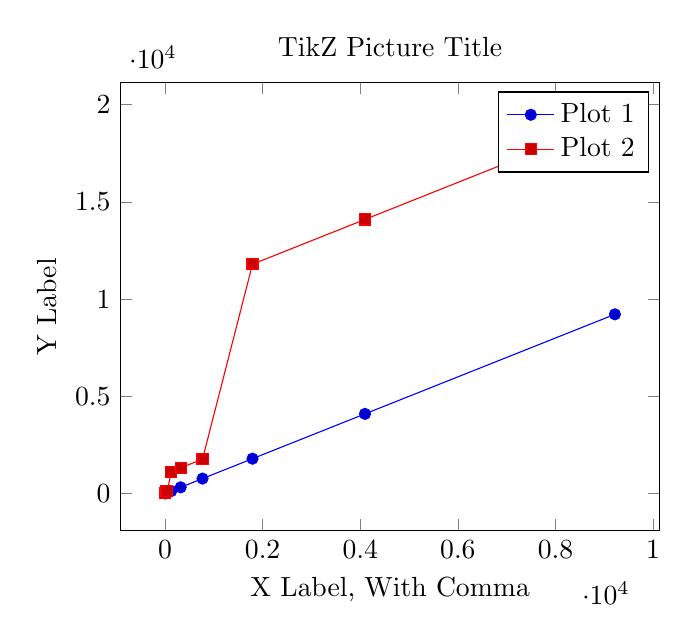
\begin{tikzpicture}
        \begin{axis}[xlabel={
            X Label, With Comma}, 
            ylabel=Y Label, 
            title=TikZ Picture Title
        ]
        \addplot coordinates {
            (5, 6)
            (17, 18)
            (49, 50)
            (129, 130)
            (321, 322)
            (769, 770)
            (1793, 1794)
            (4097, 4098)
            (9217, 9218)
        };
        \addplot coordinates {
            (5, 16)
            (17, 118)
            (49, 150)
            (129, 1130)
            (321, 1322)
            (769, 1770)
            (1793, 11794)
            (4097, 14098)
            (9217, 19218)
        };
        \legend{Plot 1, Plot 2}
        \end{axis}
    \end{tikzpicture}
    \caption{Figure Caption}
\end{figure}

\begin{figure}[h]
    \centering
    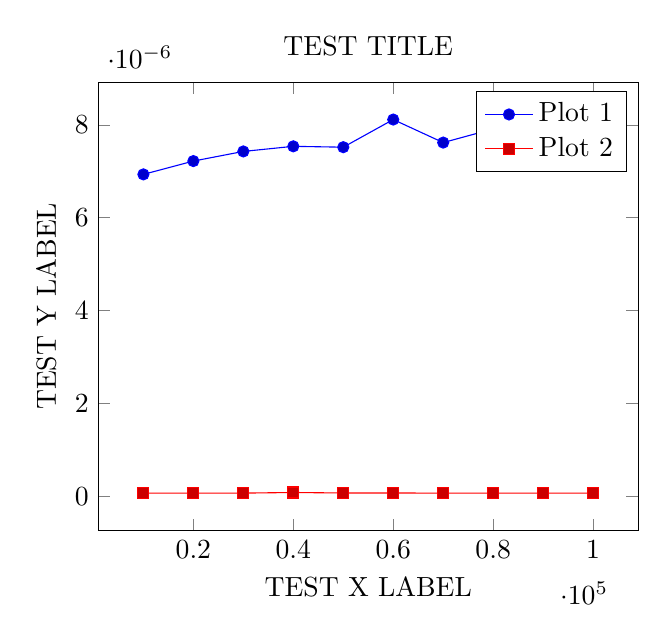
\begin{tikzpicture}
        \begin{axis}[
            xlabel={TEST X LABEL},
            ylabel={TEST Y LABEL},
            title={TEST TITLE}
        ]
		\addplot coordinates {
			(10000, 6.933658602697013e-06)
			(20000, 7.219775172611076e-06)
			(30000, 7.427586154969745e-06)
			(40000, 7.537515152884033e-06)
			(50000, 7.5188422820053894e-06)
			(60000, 8.11396474742665e-06)
			(70000, 7.618230143133564e-06)
			(80000, 7.911574921129593e-06)
			(90000, 7.978737021225424e-06)
			(100000, 7.994096963399588e-06)
		};
		\addplot coordinates {
			(10000, 7.167973014698959e-08)
			(20000, 7.167973014698959e-08)
			(30000, 7.198090548321545e-08)
			(40000, 8.523262030069035e-08)
			(50000, 7.408913284079333e-08)
			(60000, 7.439030817746329e-08)
			(70000, 7.137855480987553e-08)
			(80000, 7.137855481031963e-08)
			(90000, 7.137855480987553e-08)
			(100000, 7.107737947364967e-08)
		};
        \legend{Plot 1, Plot 2}
        \end{axis}
    \end{tikzpicture}
    \caption{TEST CAPTION}
\end{figure}

\end{document}
